\begin{figure}
    \centering
    \captionsetup[subfigure]{labelformat=empty}
\begin{subfigure}{.5\textwidth}
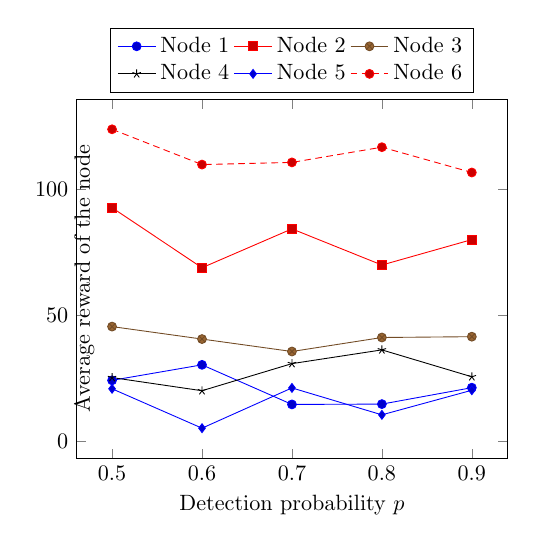
\begin{tikzpicture}[scale=0.8]
\begin{axis}[
  xlabel={Detection probability $p$},
  ylabel={Average reward of the node },
  y label style={at={(0.06,0.5)}},
  xtick={0.5,0.6,0.7,0.8,0.9,1.0},
  legend style={at={(0.5,1.2)},cells={align=right}, anchor=north,legend columns=3},
  grid style=dashed,
]
\addplot+[]
    coordinates {
(0.5,24.2596903238)(0.6,30.4098004181)(0.7,14.7157392372)(0.8,14.8410159329)(0.9,21.3512325325)
};

\addplot+[]
    coordinates {
(0.5,92.6967638225)(0.6,68.892572501)(0.7,84.3050837463)(0.8,69.9668923619)(0.9,80.051680541)
};

\addplot+[]
    coordinates {
(0.5,45.5695982478)(0.6,40.6246377658)(0.7,35.692885081)(0.8,41.2436256503)(0.9,41.5670235599)
};

\addplot+[]
    coordinates {
(0.5,25.3670893308)(0.6,20.1438895136)(0.7,30.888009803)(0.8,36.3312849347)(0.9,25.6728772368)
};

\addplot+[]
    coordinates {
(0.5,20.9174008986)(0.6,5.30161144168)(0.7,21.2602459651)(0.8,10.5837610733)(0.9,20.3331330431)
};

\addplot+[]
    coordinates {
(0.5,123.776293271)(0.6,109.788318837)(0.7,110.653974948)(0.8,116.685625909)(0.9,106.649803871)
};

\legend{Node 1, Node 2, Node 3, Node 4, Node 5, Node 6}
\end{axis}
\end{tikzpicture}

\caption{Scenario e)}
\label{fig:nodeimp_topo2_single}
\end{subfigure}
\begin{subfigure}{.33\textwidth}
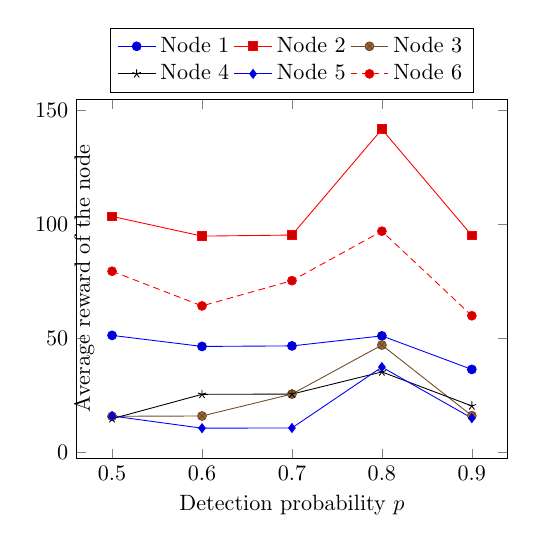
\begin{tikzpicture}[scale=0.8]
\begin{axis}[
  xlabel={Detection probability $p$},
  ylabel={Average reward of the node },
  y label style={at={(0.06,0.5)}},
  xtick={0.5,0.6,0.7,0.8,0.9,1.0},
  legend style={at={(0.5,1.2)},cells={align=right}, anchor=north,legend columns=3},
  grid style=dashed,
]

\addplot+[]
    coordinates {
(0.5,51.2408756424)(0.6,46.3989088055)(0.7,46.629281859)(0.8,51.0165854846)(0.9,36.3262102772)
};

\addplot+[]
    coordinates {
(0.5,103.390154828)(0.6,94.7445634867)(0.7,95.2136135648)(0.8,141.564157095)(0.9,95.0544799628)
};

\addplot+[]
    coordinates {
(0.5,15.7876437463)(0.6,15.9058652472)(0.7,25.5235856726)(0.8,47.0026051031)(0.9,16.0455657836)
};

\addplot+[]
    coordinates {
(0.5,14.6911918445)(0.6,25.4076999562)(0.7,25.5090975344)(0.8,35.2122191081)(0.9,20.3233753667)
};

\addplot+[]
    coordinates {
(0.5,15.9163072098)(0.6,10.573393829)(0.7,10.6704256682)(0.8,37.3424358141)(0.9,14.9838488261)
};

\addplot+[]
    coordinates {
(0.5,79.3520830459)(0.6,64.1507914239)(0.7,75.2190374666)(0.8,96.912552594)(0.9,59.8478399229)
};

\legend{Node 1, Node 2, Node 3, Node 4, Node 5, Node 6}
\end{axis}
\end{tikzpicture}

\caption{Scenario f)}
\label{fig:nodeimp_topo2_multiple}
\end{subfigure}
\caption{Results for single and multiple attackers - Scenarios e) and f)}
    \label{fig:mdp-result-topo2}
\end{figure}